\textit{Machine learning} (ML) é uma sub área da inteligência artificial voltada à otimizar critérios de desempenho de acordo com análise de dados e ocorrências passadas. \cite{alpaydin2010} Uma das características mais marcantes da ML é a análise de \textit{datasets} para automatizar o desenvolvimento de modelos analíticos para suas funcionalidades, isso quer dizer que de acordo com essas análises e com dados de ocorrências já conhecidas por uma aplicação baseada em ML, o aprendizado possibilita às aplicações reagirem de maneira autônoma à eventualidades para as quais não foram programadas.

\textit{Machine Learning} normalmente é utilizada em duas situações que podem ser enchergadas pela análise do problema:

\begin{itemize}
    \item Complexidade elevada do problema: \\ Por exemplo, tarefas rotineiras que seres humanos executam, mas que para serem programadas o algorítmo teria uma complexitade enorme como dirigir ou reconhecer imagens. Outro exemplo é a necessidade de um processamento de uma massa de dados muito grande.
    \item Necessidade de adaptabilidade do sistema: \\ Por exemplo, detecção de diversos tipos de spam, para marcar mensagens. \\ \cite{shalev2014}
\end{itemize}

\subsection{\textit{Workflow}}
    O \textit{workflow} básico de ML consiste em duas fases, a de construção de um modelo e a de predição. Na primeira são utilizados dados históricos (ou dados de treinamento) para um ciclo de modelagem de dados onde será definido, evoluido e otimizado um modelo de dados para que o algorítmo o consuma, realizando assim um tipo de aprendizado. É a partir deste modelo otmizado que o algorítmo vai conseguir fazer predições sobre novos dados ou ainda categorizações.

    \begin{figure}[ht]
            \centering
            \label{fig06}
                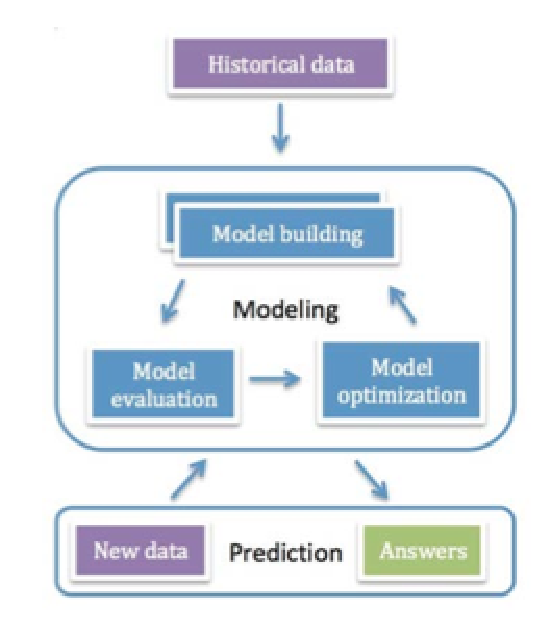
\includegraphics[keepaspectratio=true, scale=0.7]{editaveis/images/mlworkflow.eps}
            \caption{\textit{Workflow} básico de ML.}
            Fonte : \cite{brink2015}
    \end{figure}

\subsection{Tipos de aprendizado}
    \begin{itemize}
        \item Supervisionado: No aprendizado supervisionado, uma massa de dados de treinamento é rodada pelo programa possuindo labels características que as classificam, e no momento em que um novo dado aparece sem essa label (dado de teste), espera-se que o programa seja capaz de predizer qual a classificação do dado.
        \item Não Supervisionado: No aprendizado não supervisionado, a massa de dados de treinamento é a mesma dos dados de teste, pois estes dados não possuem labels que distingüem características. Dessa forma o programa reconhece as características a cada novo dado entregue e começa a fazer a separação de forma autonoma. \cite{chao2011}
        \item Reforço: No aprendizado por reforço, o programa ao receber um sinal de entrada dispara uma ação que muda o valor deste sinal. Assim que o valor do sinal de entrada é alterado e devolvido, mudando assim o estado do ambiente de aprendizagem. A partir disso é recebida uma nova entrada para disparar outra ação que novamente devolverá um valor diferente alterando o estado do ambiente, com a intenç!ao de sempre se aumentar os valores de interação. \cite{kaelbling1996}
    \end{itemize}



